\mychapter{Projeto SpaceVANT}
\label{Cap:SpaceVANT}

Como mencionado anteriormente, o projeto SpaceVANT é um projeto pela Universidade Federal do Rio Grande do Norte (UFRN), mais precisamente alocado no Departamento de Engenharia da Computação e Automação, em parceria com o Centro de Lançamento Barreira do Inferno (CLBI). O projeto tem por objetivo tornar o processo de verificação da área de impacto de foguetes lançados pelo CLBI mais eficiente tanto em relação ao tempo gasto quanto ao custo financeiro \cite{everaerts2008use}.

\section{Solução Atual}

Atualmente, a área de impacto de um foguete a ser lançado é vistoriado com o auxílio de um avião tripulado que sobrevoa a área em busca de embarcações não autorizadas. Somente quando o avião sobrevoa toda a região e certifica que nenhum embarcação se encontra no local, só então o lançamento poderá ser autorizado.

Essa solução sendo empregada no momento possui alguns pontos negativos, primeiramente, o custo com os aviões que realizarão a operação de varredura, bem como o custo de manutenção dos mesmo, é bastante elevado quando comparado com o custo de aquisição e manutenção de VANTs. Além disso, a depender do tamanho da área a ser vistoriada, o emprego de mais de um avião pode ser necessário para garantir que não haverá nenhuma embarcação não autorizada no período de tempo determinado pela missão, dessa forma, aumentando ainda mais o custo da operação.

\section{Objetivo do Projeto}


Visando, então, solucionar o problema acima apresentado de forma mais eficaz, o projeto SpaceVANT visa desenvolver sistema de VANTs autónomos que irão realizar a varredura da área de impacto que será entrada do sistema supervisório da solução.

O produto final do projeto incluirá: um sistema supervisório ou estação base, aeronaves autónomas do modelo \emph{Penguin} (Fig \ref{fig:penguin}) dotadas de computador e câmera fotografica embarcados e, por fim, uma rede de comunicação que conectará todas a aeronaves e a estação base. 

\begin{figure} 
\center
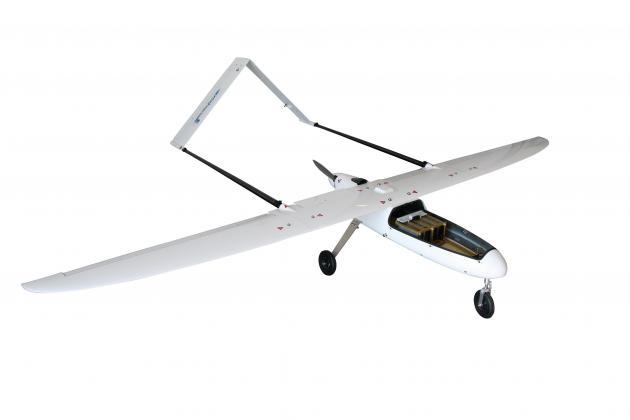
\includegraphics[width=0.7\textwidth]{penguin.jpg}
\caption{Aeronave modelo Penguin.} 
\label{fig:penguin}
\end{figure}

Para a realização da missão de varredura serão necessários algumas entradas a estação base, sendo elas, a quantidade de aeronaves a serem empregadas na missão, tempo de duração da missão, área a ser varrida e estratégia de varredura a ser utilizada, estratégias essas que serão apresentadas no Cap. \ref{Cap:Estrategia}.

Quando fornecidas todas as entradas corretamente, as rotas de voo serão definidas e carregadas nos VANTs e a missão terá inicio. O progresso da missão poderá ser acompanhada através da estação base e caso alguma embarcação seja identificada um alerta será lançado pela rede ate chegar a estação base visível ao operador da missão. Esse alerta será composto pela imagem da possível embarcação identificada pelo sistema, a localização geográfica do objeto e a hora na qual ele foi identificado.  






 